% answers.tex —— 1985 年·全国卷·理科 · 参考答案与详细解析片段
% 由 tools/generate_projects.py 依来源总账自 1985/1985_数学真题_全国理_试题.md + 1985/1985_数学真题_全国理_解析正文.md + 1985/1985_数学真题_全国理_答案要点.md 生成，勿手改（改源 MD 后重跑）


\begin{gktip}
固定源只有一页题面，不含答案。以下逐题给出本库独立推导；复杂图形题按原图关系重绘为 TikZ 矢量图，答案结论不宣称为官方发布版本。
\end{gktip}

\begin{answer}
\gksolhead{1}{}

\textbf{题目}：

\Needspace{5\baselineskip}
如果正方体 $ABCD-A'B'C'D'$ 的棱长为 $a$，那么四面体 $A'-ABD$ 的体积是\mbox{（　　）}

\nopagebreak[4]
\[
\text{（A）}\ \frac{a^3}{2}
\qquad
\text{（B）}\ \frac{a^3}{3}
\qquad
\text{（C）}\ \frac{a^3}{4}
\qquad
\text{（D）}\ \frac{a^3}{6}
\]

\Needspace{4\baselineskip}
\textbf{解析}

\Needspace{5\baselineskip}
三角形 $ABD$ 是边长为 $a$ 的等边三角形，面积为 $\frac12a^2$；点 $A'$ 到底面 $ABD$ 的高为 $AA'=a$。所以

\nopagebreak[4]
\[
V_{A'-ABD}=\frac13\cdot\frac12a^2\cdot a=\frac{a^3}{6}.
\]

故选（D）。

\gkanswer{答案：（D）$\dfrac{a^3}{6}$}

\end{answer}
\begin{answer}
\gksolhead{2}{}

\textbf{题目}：

$\tan x=1$ 是 $x=\dfrac54\pi$ 的\mbox{（　　）}

（A）必要条件　　（B）充分条件　　（C）充分必要条件　　（D）既不充分又不必要的条件

\Needspace{4\baselineskip}
\textbf{解析}

\Needspace{5\baselineskip}
$x=\frac54\pi$ 能推出 $\tan x=1$，但 $\tan x=1$ 的解为

\nopagebreak[4]
\[
x=\frac\pi4+k\pi,\qquad k\in\mathbb Z,
\]

并不必然等于 $\frac54\pi$。因此“$\tan x=1$”是“$x=\frac54\pi$”的必要条件，选（A）。

\gkanswer{答案：（A）必要条件}

\end{answer}
\begin{answer}
\gksolhead{3}{}

\textbf{题目}：

在下面给出的函数中，哪一个函数既是区间 $\left(0,\dfrac\pi2\right)$ 上的增函数又是以 $\pi$ 为周期的偶函数\mbox{（　　）}

（A）$y=x^2\ (x\in\mathbb R)$

（B）$y=|\sin x|\ (x\in\mathbb R)$

（C）$y=\cos2x\ (x\in\mathbb R)$

（D）$y=e^{\sin2x}\ (x\in\mathbb R)$

\Needspace{4\baselineskip}
\textbf{解析}

\Needspace{5\baselineskip}
$|\sin x|$ 是偶函数，且

\nopagebreak[4]
\[
|\sin(x+\pi)|=|-\sin x|=|\sin x|,
\]

所以它以 $\pi$ 为周期。在 $\left(0,\frac\pi2\right)$ 上，$\sin x$ 严格递增，故 $|\sin x|=\sin x$ 也严格递增。

其余选项分别因不具 $\pi$ 周期、在该区间递减或不为偶函数而不合题意。故选（B）。

\gkanswer{答案：（B）$y=|\sin x|$}

\end{answer}
\begin{answer}
\gksolhead{4}{}

\textbf{题目}：

\Needspace{5\baselineskip}
极坐标方程

\nopagebreak[4]
\[
\rho=a\sin\theta\qquad(a>0)
\]

的图象是\mbox{（　　）}
\nopagebreak[4]
\begin{center}% 1985 年全国卷理科第 4 题：极坐标方程 rho=a sin(theta) 的四个选项
\begin{tikzpicture}[scale=0.62,>=stealth]
  \begin{scope}[shift={(0,1.55)}]
    \draw[->] (-1.15,0)--(1.65,0) node[right] {$x$};
    \node[above left] at (-1.0,0.02) {$O$};
    \draw (0.34,0) circle (0.78);
    \fill (0.34,0) circle (1pt) node[below] {$\frac a2$};
    \node[below] at (0,-1.15) {（A）};
  \end{scope}
  \begin{scope}[shift={(3.0,1.55)}]
    \draw[->] (-1.15,0)--(1.65,0) node[right] {$x$};
    \node[above left] at (-1.0,0.02) {$O$};
    \draw (0.75,0) circle (1.12);
    \fill (0.75,0) circle (1pt) node[below] {$a$};
    \node[below] at (0,-1.15) {（B）};
  \end{scope}
  \begin{scope}[shift={(0,-1.55)}]
    \draw[->] (-1.15,0)--(1.65,0) node[right] {$x$};
    \node[above left] at (-1.0,0.02) {$O$};
    \draw (0,0.78) circle (0.78);
    \fill (0,0.78) circle (1pt) node[right] {$\frac a2$};
    \draw (0,0)--(0,0.78);
    \node[below] at (0,-1.15) {（C）};
  \end{scope}
  \begin{scope}[shift={(3.0,-1.55)}]
    \draw[->] (-1.15,0)--(1.65,0) node[right] {$x$};
    \node[above left] at (-1.0,0.02) {$O$};
    \draw (0,1.05) circle (1.05);
    \fill (0,1.05) circle (1pt) node[right] {$a$};
    \draw (0,0)--(0,1.05);
    \node[below] at (0,-1.15) {（D）};
  \end{scope}
\end{tikzpicture}
\end{center}
\nopagebreak[4]
\Needspace{4\baselineskip}
\textbf{解析}

由极坐标与直角坐标的关系 $x=\rho\cos\theta$、$y=\rho\sin\theta$，将
\Needspace{5\baselineskip}
$\rho=a\sin\theta$ 两边乘以 $\rho$ 得

\nopagebreak[4]
\[
\rho^2=a\rho\sin\theta,
\qquad
x^2+y^2=ay.
\]

\Needspace{5\baselineskip}
配方为

\nopagebreak[4]
\[
x^2+\left(y-\frac a2\right)^2=\left(\frac a2\right)^2.
\]

这是圆心在 $(0,a/2)$、半径为 $a/2$ 的圆，经过原点且与 $x$ 轴相切。故选（C）。

\gkanswer{答案：（C）}

\end{answer}
\begin{answer}
\gksolhead{5}{}

\textbf{题目}：

用 $1,2,3,4,5$ 这五个数字，可以组成比 $20000$ 大，并且百位数不是数字 $3$ 的没有重复数字的五位数，共有\mbox{（　　）}

（A）96 个　　（B）78 个　　（C）72 个　　（D）64 个

\Needspace{4\baselineskip}
\textbf{解析}

五位数必须把 $1,2,3,4,5$ 各使用一次。首位为 $2\text{、}3\text{、}4\text{、}5$ 才可能大于 $20000$。

\Needspace{5\baselineskip}
首位为 $2\text{、}4\text{、}5$ 时，剩余数字中有 $3$，百位不能取 $3$，百位有 $3$ 种取法，其他三位有 $3!$ 种排列，共

\nopagebreak[4]
\[
3\times3\times3!=54
\]

\Needspace{5\baselineskip}
种。首位为 $3$ 时，剩余数字不含 $3$，百位有 $4$ 种取法，其他三位有 $3!$ 种排列，共

\nopagebreak[4]
\[
4\times3!=24
\]

\Needspace{5\baselineskip}
种。因此总数为

\nopagebreak[4]
\[
54+24=78.
\]

故选（B）。

\gkanswer{答案：（B）$78$ 个}

\end{answer}
\begin{answer}
\gksolhead{6}{}

\textbf{题目}：

\Needspace{5\baselineskip}
求方程

\nopagebreak[4]
\[
2\sin\left(x+\frac\pi6\right)=1
\]

的解集。

\Needspace{4\baselineskip}
\textbf{解析}

\Needspace{5\baselineskip}
令 $t=x+\frac\pi6$，则 $\sin t=\frac12$，所以

\nopagebreak[4]
\[
t=\frac\pi6+2k\pi
\quad\text{\text{或}}\quad
t=\frac{5\pi}{6}+2k\pi,
\qquad k\in\mathbb Z.
\]

\Needspace{5\baselineskip}
从而

\nopagebreak[4]
\[
x=2k\pi
\quad\text{\text{或}}\quad
x=\frac{2\pi}{3}+2k\pi,
\qquad k\in\mathbb Z.
\]

\gkanswer{答案：$x=2k\pi$ 或 $x=\dfrac{2\pi}{3}+2k\pi$，$k\in\mathbb Z$}

\end{answer}
\begin{answer}
\gksolhead{7}{}

\textbf{题目}：

\Needspace{5\baselineskip}
设 $|a|\le1$，求

\nopagebreak[4]
\[
\arccos a+\arccos(-a)
\]

的值。

\Needspace{4\baselineskip}
\textbf{解析}

\Needspace{5\baselineskip}
由于 $|a|\le1$，反余弦函数的值域为 $[0,\pi]$，并且

\nopagebreak[4]
\[
\arccos(-a)=\pi-\arccos a.
\]

\Needspace{5\baselineskip}
因此

\nopagebreak[4]
\[
\arccos a+\arccos(-a)=\pi.
\]

\gkanswer{答案：$\pi$}

\end{answer}
\begin{answer}
\gksolhead{8}{}

\textbf{题目}：

\Needspace{5\baselineskip}
求曲线

\nopagebreak[4]
\[
y^2=-16x+64
\]

的焦点。

\Needspace{4\baselineskip}
\textbf{解析}

\Needspace{5\baselineskip}
配方为

\nopagebreak[4]
\[
y^2=-16(x-4).
\]

\Needspace{5\baselineskip}
与标准式 $y^2=4p(x-4)$ 比较，得 $4p=-16$，即 $p=-4$。焦点为

\nopagebreak[4]
\[
(4+p,0)=(0,0).
\]

\gkanswer{答案：$(0,0)$}

\end{answer}
\begin{answer}
\gksolhead{9}{}

\textbf{题目}：

\Needspace{5\baselineskip}
设

\nopagebreak[4]
\[
(3x-1)^6=a_6x^6+a_5x^5+a_4x^4+a_3x^3+a_2x^2+a_1x+a_0,
\]

求 $a_6+a_5+a_4+a_3+a_2+a_1+a_0$ 的值。

\Needspace{4\baselineskip}
\textbf{解析}

\Needspace{5\baselineskip}
令 $x=1$，则多项式左端为 $(3-1)^6$，右端为系数之和。因此

\nopagebreak[4]
\[
a_6+a_5+a_4+a_3+a_2+a_1+a_0=2^6=64.
\]

\gkanswer{答案：$64$}

\end{answer}
\begin{answer}
\gksolhead{10}{}

\textbf{题目}：

设函数 $f(x)$ 的定义域是 $[0,1]$，求函数 $f(x^2)$ 的定义域。

\Needspace{4\baselineskip}
\textbf{解析}

\Needspace{5\baselineskip}
$f(x^2)$ 有定义当且仅当 $x^2$ 落在 $f$ 的定义域 $[0,1]$ 中，即

\nopagebreak[4]
\[
0\le x^2\le1.
\]

\Needspace{5\baselineskip}
故 $-1\le x\le1$，定义域为

\nopagebreak[4]
\[
[-1,1].
\]

\gkanswer{答案：$[-1,1]$}

\end{answer}
\begin{answer}
\gksolhead{11}{}

\textbf{题目}：

\Needspace{5\baselineskip}
解方程：

\nopagebreak[4]
\[
\log_4(3-x)+\log_{0.25}(3+x)
=\log_4(1-x)+\log_{0.25}(2x+1).
\]

\Needspace{4\baselineskip}
\textbf{解析}

\Needspace{5\baselineskip}
定义域要求

\nopagebreak[4]
\[
3-x>0,\quad 3+x>0,\quad 1-x>0,\quad 2x+1>0,
\]

\Needspace{5\baselineskip}
所以 $-\frac12<x<1$。又因为 $\log_{0.25}u=-\log_4u$，原方程化为

\nopagebreak[4]
\[
\log_4\frac{3-x}{3+x}
=\log_4\frac{1-x}{2x+1}.
\]

\Needspace{5\baselineskip}
于是

\nopagebreak[4]
\[
(3-x)(2x+1)=(3+x)(1-x),
\]

\Needspace{5\baselineskip}
化简得

\nopagebreak[4]
\[
x(x-7)=0.
\]

只有 $x=0$ 在定义域内，故解为 $x=0$。

\gkanswer{答案：$x=0$}

\end{answer}
\begin{answer}
\gksolhead{12}{}

\textbf{题目}：

\Needspace{5\baselineskip}
解不等式：

\nopagebreak[4]
\[
\sqrt{2x+5}>x+1.
\]

\Needspace{4\baselineskip}
\textbf{解析}

定义域为 $x\ge-\frac52$。当 $x<-1$ 时，右端 $x+1<0$，而左端非负，不等式自动成立。

\Needspace{5\baselineskip}
当 $x\ge-1$ 时两边非负，可以平方：

\nopagebreak[4]
\[
2x+5>(x+1)^2
\quad\Longleftrightarrow\quad
x^2<4.
\]

\Needspace{5\baselineskip}
与 $x\ge-1$ 合并得 $-1\le x<2$，所以解集为

\nopagebreak[4]
\[
\left[-\frac52,-1\right)\cup[-1,2)
=\left[-\frac52,2\right).
\]

\gkanswer{答案：$x\in\left[-\dfrac52,2\right)$}

\end{answer}
\begin{answer}
\gksolhead{13}{}

\textbf{题目}：

如图，设平面 $AC$ 和 $BD$ 相交于 $BC$，它们所成的一个二面角为 $45^\circ$，$P$ 为平面 $AC$ 内的一点，$Q$ 为平面 $BD$ 内的一点。已知直线 $MQ$ 是直线 $PQ$ 在平面 $BD$ 内的射影，并且 $M$ 在 $BC$ 上。又设 $PQ$ 与平面 $BD$ 所成的角为 $\beta$，$\angle CMQ=\theta$（$0^\circ<\theta<90^\circ$），线段 $PM$ 的长为 $a$，求线段 $PQ$ 的长。

\begin{gktip}
原源 PDF 第 1 页附有两个相交平面、点 $P,Q,M$ 及投影线段的示意图；LaTeX 版按源图关系重绘。
\end{gktip}
\nopagebreak[4]
\begin{center}% 1985 年全国卷理科第 13 题：两个相交平面及投影关系
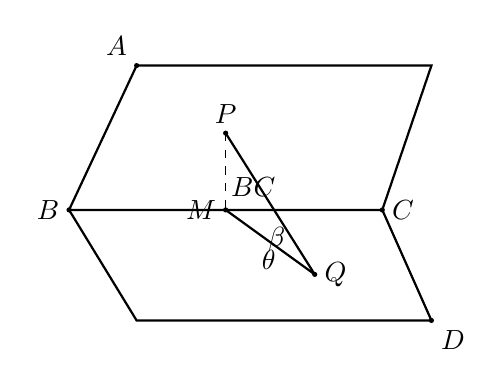
\begin{tikzpicture}[scale=0.78]
  \coordinate (B) at (0,0);
  \coordinate (C) at (5.1,0);
  \coordinate (A) at (1.1,2.35);
  \coordinate (E) at (5.9,2.35);
  \coordinate (F) at (1.1,-1.8);
  \coordinate (D) at (5.9,-1.8);
  \coordinate (P) at (2.55,1.25);
  \coordinate (M) at (2.55,0);
  \coordinate (Q) at (4.0,-1.05);
  \draw[thick] (B)--(A)--(E)--(C)--cycle;
  \draw[thick] (B)--(F)--(D)--(C);
  \draw[thick] (B)--(C);
  \draw[dashed] (P)--(M);
  \draw[thick] (P)--(Q);
  \draw[thick] (M)--(Q);
  \fill (A) circle (1.2pt) node[above left] {$A$};
  \fill (B) circle (1.2pt) node[left] {$B$};
  \fill (C) circle (1.2pt) node[right] {$C$};
  \fill (D) circle (1.2pt) node[below right] {$D$};
  \fill (P) circle (1.2pt) node[above] {$P$};
  \fill (M) circle (1.2pt) node[left] {$M$};
  \fill (Q) circle (1.2pt) node[right] {$Q$};
  \node at (3.0,0.38) {$BC$};
  \node at (3.38,-0.48) {$\beta$};
  \node at (3.25,-0.82) {$\theta$};
\end{tikzpicture}
\end{center}
\nopagebreak[4]
\Needspace{4\baselineskip}
\textbf{解析}

\Needspace{5\baselineskip}
因为 $MQ$ 是 $PQ$ 在平面 $BD$ 内的射影，且 $Q$ 已在平面 $BD$ 内，所以 $PM$ 垂直于平面 $BD$，$\triangle PMQ$ 在 $M$ 点为直角。直线与平面所成的角等于直线与其射影所成的角，因此

\nopagebreak[4]
\[
\angle PQM=\beta.
\]

\Needspace{5\baselineskip}
在直角三角形 $PMQ$ 中，

\nopagebreak[4]
\[
\sin\beta=\frac{PM}{PQ}=\frac a{PQ}.
\]

\Needspace{5\baselineskip}
故

\nopagebreak[4]
\[
PQ=\frac a{\sin\beta}.
\]

题面给出的二面角 $45^\circ$ 和 $\angle CMQ=\theta$ 保留在题设中，但在已知 $PM=a$、投影角为 $\beta$ 的直接求长关系中不再额外出现。

\gkanswer{答案：$PQ=\dfrac{a}{\sin\beta}$}

\end{answer}
\begin{answer}
\gksolhead{14}{}

\textbf{题目}：

设 $O$ 为复平面的原点，$Z_1$ 和 $Z_2$ 为复平面内的两动点，并且满足：

（1） $Z_1$ 和 $Z_2$ 所对应的复数的辐角分别为定值 $\theta$ 和 $-\theta$（$0<\theta<\dfrac\pi2$）；

（2） $\triangle OZ_1Z_2$ 的面积为定值 $S$。

求 $\triangle OZ_1Z_2$ 的重心 $Z$ 所对应的复数的模的最小值。

\Needspace{4\baselineskip}
\textbf{解析}

\gksubpart{（1）}

\Needspace{5\baselineskip}
令

\nopagebreak[4]
\[
|Z_1|=r_1,\qquad |Z_2|=r_2.
\]

\Needspace{5\baselineskip}
由于两个辐角分别为 $\theta$ 和 $-\theta$，夹角为 $2\theta$，面积条件给出

\nopagebreak[4]
\[
\frac12r_1r_2\sin2\theta=S,
\qquad
r_1r_2=\frac{2S}{\sin2\theta}.
\]

\gksubpart{（2）}

\Needspace{5\baselineskip}
重心 $Z$ 对应的复数为 $(z_1+z_2)/3$，因此

\nopagebreak[4]
\[
\begin{aligned}
|z_1+z_2|^2
&=r_1^2+r_2^2+2r_1r_2\cos2\theta\\
&=(r_1-r_2)^2+2r_1r_2(1+\cos2\theta)\\
&\ge4r_1r_2\cos^2\theta.
\end{aligned}
\]

\Needspace{5\baselineskip}
等号在 $r_1=r_2$ 时成立。代入面积条件：

\nopagebreak[4]
\[
|z_1+z_2|^2
\ge\frac{8S\cos^2\theta}{\sin2\theta}
=4S\cot\theta.
\]

\Needspace{5\baselineskip}
所以重心对应复数的模的最小值为

\nopagebreak[4]
\[
|z|_{\min}=\frac13|z_1+z_2|_{\min}
=\frac23\sqrt{S\cot\theta}.
\]

\gkanswer{答案（1）：见解析版}

\gkanswer{答案（2）：$\dfrac23\sqrt{S\cot\theta}$}

\end{answer}
\begin{answer}
\gksolhead{15}{}

\textbf{题目}：

\Needspace{5\baselineskip}
已知两点 $P(-2,2)$、$Q(0,2)$ 以及一条直线

\nopagebreak[4]
\[
L:y=x,
\]

设长为 $\sqrt2$ 的线段 $AB$ 在直线 $L$ 上移动，如图，求直线 $PA$ 和 $QB$ 的交点 $M$ 的轨迹方程。（要求把结果写成普通方程。）

\begin{gktip}
原源 PDF 第 1 页附有 $P,Q$、直线 $y=x$、可动线段 $AB$ 和交点 $M$ 的示意图；LaTeX 版按源图关系重绘。
\end{gktip}
\nopagebreak[4]
\begin{center}% 1985 年全国卷理科第 15 题：线段 AB 在 y=x 上移动
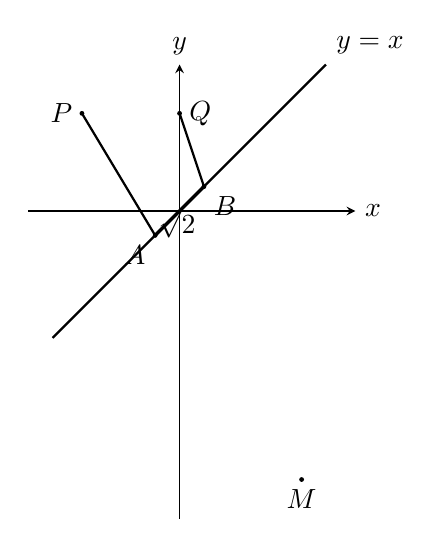
\begin{tikzpicture}[scale=0.62,>=stealth]
  \draw[->] (-3.1,0)--(3.6,0) node[right] {$x$};
  \draw[->] (0,-6.3)--(0,3.0) node[above] {$y$};
  \draw[thick] (-2.6,-2.6)--(3.0,3.0) node[above right] {$y=x$};
  \coordinate (P) at (-2,2);
  \coordinate (Q) at (0,2);
  \coordinate (A) at (-0.5,-0.5);
  \coordinate (B) at (0.5,0.5);
  \coordinate (M) at (2.5,-5.5);
  \draw[thick] (P)--(A);
  \draw[thick] (Q)--(B);
  \draw[very thick] (A)--(B);
  \fill (P) circle (1.4pt) node[left] {$P$};
  \fill (Q) circle (1.4pt) node[right] {$Q$};
  \fill (A) circle (1.4pt) node[below left] {$A$};
  \fill (B) circle (1.4pt) node[below right] {$B$};
  \fill (M) circle (1.4pt) node[below] {$M$};
  \node at (-0.05,-0.25) {$\sqrt2$};
\end{tikzpicture}
\end{center}
\nopagebreak[4]
\Needspace{4\baselineskip}
\textbf{解析}

\Needspace{5\baselineskip}
取参数 $t$，令

\nopagebreak[4]
\[
A=(t,t),\qquad B=(t+1,t+1),
\]

\Needspace{5\baselineskip}
则 $AB=\sqrt2$，并且 $A$ 在 $B$ 的左侧，正如原图标记。直线 $PA$ 和 $QB$ 的方程分别可写为

\nopagebreak[4]
\[
y-2=\frac{t-2}{t+2}(x+2),
\qquad
y-2=\frac{t-1}{t+1}x.
\]

\Needspace{5\baselineskip}
联立得到交点 $M=(x,y)$：

\nopagebreak[4]
\[
x=t-1-\frac2t,\qquad
y=t-1+\frac2t,
\qquad t\ne0.
\]

\Needspace{5\baselineskip}
于是

\nopagebreak[4]
\[
x+y+2=2t,\qquad x-y=-\frac4t.
\]

\Needspace{5\baselineskip}
消去 $t$：

\nopagebreak[4]
\[
(x-y)(x+y+2)=-8.
\]

\Needspace{5\baselineskip}
写成普通方程为

\nopagebreak[4]
\[
x^2-y^2+2x-2y+8=0,
\]

\Needspace{5\baselineskip}
或

\nopagebreak[4]
\[
(y+1)^2-(x+1)^2=8.
\]

因此轨迹是一条以 $(-1,-1)$ 为中心的等轴双曲线。

\gkanswer{答案：$x^2-y^2+2x-2y+8=0$，即 $(y+1)^2-(x+1)^2=8$}

\end{answer}
\begin{answer}
\gksolhead{16}{}

\textbf{题目}：

\Needspace{5\baselineskip}
设

\nopagebreak[4]
\[
a_n=\sqrt{1\cdot2}+\sqrt{2\cdot3}+\cdots+\sqrt{n(n+1)}
\qquad(n=1,2,\ldots).
\]

\Needspace{5\baselineskip}
（1） 证明：不等式

\nopagebreak[4]
\[
\frac{n(n+1)}2<a_n<\frac{(n+1)^2}{2}
\]

对所有的正整数 $n$ 都成立；

\Needspace{5\baselineskip}
（2） 设

\nopagebreak[4]
\[
b_n=\frac{a_n}{n(n+1)}
\qquad(n=1,2,\ldots),
\]

\Needspace{5\baselineskip}
用定义证明：

\nopagebreak[4]
\[
\lim_{n\to\infty}b_n=\frac12.
\]

\Needspace{4\baselineskip}
\textbf{解析}

\gksubpart{（1）}

\Needspace{5\baselineskip}
对每个 $k=1,2,\ldots,n$，有

\nopagebreak[4]
\[
k<\sqrt{k(k+1)}<k+\frac12,
\]

因为平方后分别得到 $k^2<k(k+1)$ 和
\Needspace{5\baselineskip}
$k(k+1)<(k+\frac12)^2$。逐项求和得

\nopagebreak[4]
\[
\frac{n(n+1)}2<a_n
<\sum_{k=1}^n\left(k+\frac12\right)
=\frac{n(n+2)}2
<\frac{(n+1)^2}{2}.
\]

所以题中的不等式对所有正整数 $n$ 成立。

\gksubpart{（2）}

\Needspace{5\baselineskip}
将（1）的不等式同除以正数 $n(n+1)$，得到

\nopagebreak[4]
\[
\frac12<
b_n
<\frac{n+1}{2n}
=\frac12+\frac1{2n}.
\]

给定任意 $\varepsilon>0$，取正整数
\Needspace{5\baselineskip}
$N>\frac1{2\varepsilon}$。当 $n>N$ 时，

\nopagebreak[4]
\[
0<b_n-\frac12<\frac1{2n}<\varepsilon.
\]

\Needspace{5\baselineskip}
这正是数列极限的 $\varepsilon$ 定义，故

\nopagebreak[4]
\[
\lim_{n\to\infty}b_n=\frac12.
\]

\gkanswer{答案（1）：见解析版}

\gkanswer{答案（2）：$\displaystyle\lim_{n\to\infty}b_n=\dfrac12$}

\end{answer}
\begin{answer}
\gksolhead{17}{}

\textbf{题目}：

\Needspace{5\baselineskip}
设 $a\text{、}b$ 是两个实数，

\nopagebreak[4]
\[
A=\{(x,y)\mid x=n,\ y=na+b,\ n\text{ \text{是整数}}\},
\]

\nopagebreak[4]
\[
B=\{(x,y)\mid x=m,\ y=3m^2+15,\ m\text{ \text{是整数}}\},
\]

\nopagebreak[4]
\[
C=\{(x,y)\mid x^2+y^2\le144\}
\]

是平面 $xOy$ 内的点集合，讨论是否存在 $a$ 和 $b$ 使得

（1） $A\cap B\ne\varnothing$（$\varnothing$ 表示空集），

（2） $(a,b)\in C$

同时成立。

\Needspace{4\baselineskip}
\textbf{解析}

\gksubpart{（1）}

\Needspace{5\baselineskip}
若 $A\cap B\ne\varnothing$，则存在整数 $n,m$ 使两点坐标相同。由横坐标得 $n=m=k$，其中 $k$ 为整数；由纵坐标得

\nopagebreak[4]
\[
ka+b=3k^2+15,
\qquad
b=3k^2+15-ka.
\]

\Needspace{5\baselineskip}
令 $c=3k^2+15$。若同时有 $(a,b)\in C$，就应有

\nopagebreak[4]
\[
a^2+b^2=a^2+(c-ka)^2\le144.
\]

\gksubpart{（2）}

\Needspace{5\baselineskip}
但二次式的最小值为

\nopagebreak[4]
\[
\min_a\{a^2+(c-ka)^2\}
=\frac{c^2}{1+k^2}.
\]

\Needspace{5\baselineskip}
注意

\nopagebreak[4]
\[
\begin{aligned}
c^2-144(1+k^2)
&=(3k^2+15)^2-144(1+k^2)\\
&=9(k^2-3)^2.
\end{aligned}
\]

\Needspace{5\baselineskip}
由于 $k$ 为整数，$k^2\ne3$，所以

\nopagebreak[4]
\[
\frac{c^2}{1+k^2}>144.
\]

这与 $(a,b)\in C$ 矛盾。因此不存在同时满足两个条件的实数 $a,b$。

\gkanswer{答案（1）：见解析版}

\gkanswer{答案（2）：不存在满足两个条件的实数 $a,b$}

\end{answer}
\begin{answer}
\gksolhead{18}{}

\textbf{题目}：

\Needspace{5\baselineskip}
已知曲线

\nopagebreak[4]
\[
y=x^3-6x^2+11x-6.
\]

在它对应于 $x\in[0,2]$ 的弧段上求一点 $P$，使得曲线在该点的切线在 $y$ 轴上的截距为最小，并求出这个最小值。

\Needspace{4\baselineskip}
\textbf{解析}

\Needspace{5\baselineskip}
设切点为

\nopagebreak[4]
\[
P=(t,f(t)),\qquad
f(t)=t^3-6t^2+11t-6,\qquad 0\le t\le2.
\]

\Needspace{5\baselineskip}
切线斜率为

\nopagebreak[4]
\[
f'(t)=3t^2-12t+11.
\]

\Needspace{5\baselineskip}
切线在 $y$ 轴上的截距为

\nopagebreak[4]
\[
\begin{aligned}
g(t)
&=f(t)-tf'(t)\\
&=-2t^3+6t^2-6.
\end{aligned}
\]

\Needspace{5\baselineskip}
其导数为

\nopagebreak[4]
\[
g'(t)=6t(2-t)\ge0\qquad(0\le t\le2),
\]

\Needspace{5\baselineskip}
所以 $g(t)$ 在 $[0,2]$ 上递增，最小值在 $t=0$ 处取得：

\nopagebreak[4]
\[
P=(0,f(0))=(0,-6),
\qquad
g(0)=-6.
\]

此时切线为 $y=11x-6$，其 $y$ 轴截距确为 $-6$。

\gkanswer{答案：$P=(0,-6)$，最小截距为 $-6$}

\end{answer}